
%% bare_conf.tex
%% V1.3
%% 2007/01/11
%% by Michael Shell
%% See:
%% http://www.michaelshell.org/
%% for current contact information.
%%
%% This is a skeleton file demonstrating the use of IEEEtran.cls
%% (requires IEEEtran.cls version 1.7 or later) with an IEEE conference paper.
%%
%% Support sites:
%% http://www.michaelshell.org/tex/ieeetran/
%% http://www.ctan.org/tex-archive/macros/latex/contrib/IEEEtran/
%% and
%% http://www.ieee.org/

%%*************************************************************************
%% Legal Notice:
%% This code is offered as-is without any warranty either expressed or
%% implied; without even the implied warranty of MERCHANTABILITY or
%% FITNESS FOR A PARTICULAR PURPOSE! 
%% User assumes all risk.
%% In no event shall IEEE or any contributor to this code be liable for
%% any damages or losses, including, but not limited to, incidental,
%% consequential, or any other damages, resulting from the use or misuse
%% of any information contained here.
%%
%% All comments are the opinions of their respective authors and are not
%% necessarily endorsed by the IEEE.
%%
%% This work is distributed under the LaTeX Project Public License (LPPL)
%% ( http://www.latex-project.org/ ) version 1.3, and may be freely used,
%% distributed and modified. A copy of the LPPL, version 1.3, is included
%% in the base LaTeX documentation of all distributions of LaTeX released
%% 2003/12/01 or later.
%% Retain all contribution notices and credits.
%% ** Modified files should be clearly indicated as such, including  **
%% ** renaming them and changing author support contact information. **
%%
%% File list of work: IEEEtran.cls, IEEEtran_HOWTO.pdf, bare_adv.tex,
%%                    bare_conf.tex, bare_jrnl.tex, bare_jrnl_compsoc.tex
%%*************************************************************************

% *** Authors should verify (and, if needed, correct) their LaTeX system  ***
% *** with the testflow diagnostic prior to trusting their LaTeX platform ***
% *** with production work. IEEE's font choices can trigger bugs that do  ***
% *** not appear when using other class files.                            ***
% The testflow support page is at:
% http://www.michaelshell.org/tex/testflow/



% Note that the a4paper option is mainly intended so that authors in
% countries using A4 can easily print to A4 and see how their papers will
% look in print - the typesetting of the document will not typically be
% affected with changes in paper size (but the bottom and side margins will).
% Use the testflow package mentioned above to verify correct handling of
% both paper sizes by the user's LaTeX system.
%
% Also note that the "draftcls" or "draftclsnofoot", not "draft", option
% should be used if it is desired that the figures are to be displayed in
% draft mode.
%
\documentclass[conference]{IEEEtran}
% Add the compsoc option for Computer Society conferences.
%
% If IEEEtran.cls has not been installed into the LaTeX system files,
% manually specify the path to it like:
% \documentclass[conference]{../sty/IEEEtran}





% Some very useful LaTeX packages include:
% (uncomment the ones you want to load)


% *** MISC UTILITY PACKAGES ***
%
%\usepackage{ifpdf}
% Heiko Oberdiek's ifpdf.sty is very useful if you need conditional
% compilation based on whether the output is pdf or dvi.
% usage:
% \ifpdf
%   % pdf code
% \else
%   % dvi code
% \fi
% The latest version of ifpdf.sty can be obtained from:
% http://www.ctan.org/tex-archive/macros/latex/contrib/oberdiek/
% Also, note that IEEEtran.cls V1.7 and later provides a builtin
% \ifCLASSINFOpdf conditional that works the same way.
% When switching from latex to pdflatex and vice-versa, the compiler may
% have to be run twice to clear warning/error messages.






% *** CITATION PACKAGES ***
%
%\usepackage{cite}
% cite.sty was written by Donald Arseneau
% V1.6 and later of IEEEtran pre-defines the format of the cite.sty package
% \cite{} output to follow that of IEEE. Loading the cite package will
% result in citation numbers being automatically sorted and properly
% "compressed/ranged". e.g., [1], [9], [2], [7], [5], [6] without using
% cite.sty will become [1], [2], [5]--[7], [9] using cite.sty. cite.sty's
% \cite will automatically add leading space, if needed. Use cite.sty's
% noadjust option (cite.sty V3.8 and later) if you want to turn this off.
% cite.sty is already installed on most LaTeX systems. Be sure and use
% version 4.0 (2003-05-27) and later if using hyperref.sty. cite.sty does
% not currently provide for hyperlinked citations.
% The latest version can be obtained at:
% http://www.ctan.org/tex-archive/macros/latex/contrib/cite/
% The documentation is contained in the cite.sty file itself.






% *** GRAPHICS RELATED PACKAGES ***
%
\ifCLASSINFOpdf
   \usepackage[pdftex]{graphicx}
  % declare the path(s) where your graphic files are
  % \graphicspath{{../pdf/}{../jpeg/}}
  % and their extensions so you won't have to specify these with
  % every instance of \includegraphics
  % \DeclareGraphicsExtensions{.pdf,.jpeg,.png}
\else
  % or other class option (dvipsone, dvipdf, if not using dvips). graphicx
  % will default to the driver specified in the system graphics.cfg if no
  % driver is specified.
  % \usepackage[dvips]{graphicx}
  % declare the path(s) where your graphic files are
  % \graphicspath{{../eps/}}
  % and their extensions so you won't have to specify these with
  % every instance of \includegraphics
  % \DeclareGraphicsExtensions{.eps}
\fi
% graphicx was written by David Carlisle and Sebastian Rahtz. It is
% required if you want graphics, photos, etc. graphicx.sty is already
% installed on most LaTeX systems. The latest version and documentation can
% be obtained at: 
% http://www.ctan.org/tex-archive/macros/latex/required/graphics/
% Another good source of documentation is "Using Imported Graphics in
% LaTeX2e" by Keith Reckdahl which can be found as epslatex.ps or
% epslatex.pdf at: http://www.ctan.org/tex-archive/info/
%
% latex, and pdflatex in dvi mode, support graphics in encapsulated
% postscript (.eps) format. pdflatex in pdf mode supports graphics
% in .pdf, .jpeg, .png and .mps (metapost) formats. Users should ensure
% that all non-photo figures use a vector format (.eps, .pdf, .mps) and
% not a bitmapped formats (.jpeg, .png). IEEE frowns on bitmapped formats
% which can result in "jaggedy"/blurry rendering of lines and letters as
% well as large increases in file sizes.
%
% You can find documentation about the pdfTeX application at:
% http://www.tug.org/applications/pdftex





% *** MATH PACKAGES ***
%
%\usepackage[cmex10]{amsmath}
% A popular package from the American Mathematical Society that provides
% many useful and powerful commands for dealing with mathematics. If using
% it, be sure to load this package with the cmex10 option to ensure that
% only type 1 fonts will utilized at all point sizes. Without this option,
% it is possible that some math symbols, particularly those within
% footnotes, will be rendered in bitmap form which will result in a
% document that can not be IEEE Xplore compliant!
%
% Also, note that the amsmath package sets \interdisplaylinepenalty to 10000
% thus preventing page breaks from occurring within multiline equations. Use:
%\interdisplaylinepenalty=2500
% after loading amsmath to restore such page breaks as IEEEtran.cls normally
% does. amsmath.sty is already installed on most LaTeX systems. The latest
% version and documentation can be obtained at:
% http://www.ctan.org/tex-archive/macros/latex/required/amslatex/math/





% *** SPECIALIZED LIST PACKAGES ***
%
%\usepackage{algorithmic}
% algorithmic.sty was written by Peter Williams and Rogerio Brito.
% This package provides an algorithmic environment fo describing algorithms.
% You can use the algorithmic environment in-text or within a figure
% environment to provide for a floating algorithm. Do NOT use the algorithm
% floating environment provided by algorithm.sty (by the same authors) or
% algorithm2e.sty (by Christophe Fiorio) as IEEE does not use dedicated
% algorithm float types and packages that provide these will not provide
% correct IEEE style captions. The latest version and documentation of
% algorithmic.sty can be obtained at:
% http://www.ctan.org/tex-archive/macros/latex/contrib/algorithms/
% There is also a support site at:
% http://algorithms.berlios.de/index.html
% Also of interest may be the (relatively newer and more customizable)
% algorithmicx.sty package by Szasz Janos:
% http://www.ctan.org/tex-archive/macros/latex/contrib/algorithmicx/




% *** ALIGNMENT PACKAGES ***
%
%\usepackage{array}
% Frank Mittelbach's and David Carlisle's array.sty patches and improves
% the standard LaTeX2e array and tabular environments to provide better
% appearance and additional user controls. As the default LaTeX2e table
% generation code is lacking to the point of almost being broken with
% respect to the quality of the end results, all users are strongly
% advised to use an enhanced (at the very least that provided by array.sty)
% set of table tools. array.sty is already installed on most systems. The
% latest version and documentation can be obtained at:
% http://www.ctan.org/tex-archive/macros/latex/required/tools/


%\usepackage{mdwmath}
%\usepackage{mdwtab}
% Also highly recommended is Mark Wooding's extremely powerful MDW tools,
% especially mdwmath.sty and mdwtab.sty which are used to format equations
% and tables, respectively. The MDWtools set is already installed on most
% LaTeX systems. The lastest version and documentation is available at:
% http://www.ctan.org/tex-archive/macros/latex/contrib/mdwtools/


% IEEEtran contains the IEEEeqnarray family of commands that can be used to
% generate multiline equations as well as matrices, tables, etc., of high
% quality.


%\usepackage{eqparbox}
% Also of notable interest is Scott Pakin's eqparbox package for creating
% (automatically sized) equal width boxes - aka "natural width parboxes".
% Available at:
% http://www.ctan.org/tex-archive/macros/latex/contrib/eqparbox/





% *** SUBFIGURE PACKAGES ***
%\usepackage[tight,footnotesize]{subfigure}
% subfigure.sty was written by Steven Douglas Cochran. This package makes it
% easy to put subfigures in your figures. e.g., "Figure 1a and 1b". For IEEE
% work, it is a good idea to load it with the tight package option to reduce
% the amount of white space around the subfigures. subfigure.sty is already
% installed on most LaTeX systems. The latest version and documentation can
% be obtained at:
% http://www.ctan.org/tex-archive/obsolete/macros/latex/contrib/subfigure/
% subfigure.sty has been superceeded by subfig.sty.



%\usepackage[caption=false]{caption}
%\usepackage[font=footnotesize]{subfig}
% subfig.sty, also written by Steven Douglas Cochran, is the modern
% replacement for subfigure.sty. However, subfig.sty requires and
% automatically loads Axel Sommerfeldt's caption.sty which will override
% IEEEtran.cls handling of captions and this will result in nonIEEE style
% figure/table captions. To prevent this problem, be sure and preload
% caption.sty with its "caption=false" package option. This is will preserve
% IEEEtran.cls handing of captions. Version 1.3 (2005/06/28) and later 
% (recommended due to many improvements over 1.2) of subfig.sty supports
% the caption=false option directly:
%\usepackage[caption=false,font=footnotesize]{subfig}
%
% The latest version and documentation can be obtained at:
% http://www.ctan.org/tex-archive/macros/latex/contrib/subfig/
% The latest version and documentation of caption.sty can be obtained at:
% http://www.ctan.org/tex-archive/macros/latex/contrib/caption/




% *** FLOAT PACKAGES ***
%
%\usepackage{fixltx2e}
% fixltx2e, the successor to the earlier fix2col.sty, was written by
% Frank Mittelbach and David Carlisle. This package corrects a few problems
% in the LaTeX2e kernel, the most notable of which is that in current
% LaTeX2e releases, the ordering of single and double column floats is not
% guaranteed to be preserved. Thus, an unpatched LaTeX2e can allow a
% single column figure to be placed prior to an earlier double column
% figure. The latest version and documentation can be found at:
% http://www.ctan.org/tex-archive/macros/latex/base/



%\usepackage{stfloats}
% stfloats.sty was written by Sigitas Tolusis. This package gives LaTeX2e
% the ability to do double column floats at the bottom of the page as well
% as the top. (e.g., "\begin{figure*}[!b]" is not normally possible in
% LaTeX2e). It also provides a command:
%\fnbelowfloat
% to enable the placement of footnotes below bottom floats (the standard
% LaTeX2e kernel puts them above bottom floats). This is an invasive package
% which rewrites many portions of the LaTeX2e float routines. It may not work
% with other packages that modify the LaTeX2e float routines. The latest
% version and documentation can be obtained at:
% http://www.ctan.org/tex-archive/macros/latex/contrib/sttools/
% Documentation is contained in the stfloats.sty comments as well as in the
% presfull.pdf file. Do not use the stfloats baselinefloat ability as IEEE
% does not allow \baselineskip to stretch. Authors submitting work to the
% IEEE should note that IEEE rarely uses double column equations and
% that authors should try to avoid such use. Do not be tempted to use the
% cuted.sty or midfloat.sty packages (also by Sigitas Tolusis) as IEEE does
% not format its papers in such ways.





% *** PDF, URL AND HYPERLINK PACKAGES ***
%
%\usepackage{url}
% url.sty was written by Donald Arseneau. It provides better support for
% handling and breaking URLs. url.sty is already installed on most LaTeX
% systems. The latest version can be obtained at:
% http://www.ctan.org/tex-archive/macros/latex/contrib/misc/
% Read the url.sty source comments for usage information. Basically,
% \url{my_url_here}.





% *** Do not adjust lengths that control margins, column widths, etc. ***
% *** Do not use packages that alter fonts (such as pslatex).         ***
% There should be no need to do such things with IEEEtran.cls V1.6 and later.
% (Unless specifically asked to do so by the journal or conference you plan
% to submit to, of course. )


% correct bad hyphenation here
\hyphenation{op-tical net-works semi-conduc-tor}


\begin{document}
%
% paper title
% can use linebreaks \\ within to get better formatting as desired
\title{Final Project Report for B553\\Face Hallucination}


% author names and affiliations
% use a multiple column layout for up to three different
% affiliations
\author{\IEEEauthorblockN{Chaitanya Bilgikar}
\IEEEauthorblockA{School of Informatics and\\Computing\\
Indiana University\\
Bloomington, Indiana 47405\\
Email: cbilgika@indiana.edu}
\and
\IEEEauthorblockN{Nasheed Moiz}
\IEEEauthorblockA{School of Informatics and\\Computing\\
Indiana University\\
Bloomoington, Indiana 47405\\
Email: nmoiz@indiana.edu}
}

% conference papers do not typically use \thanks and this command
% is locked out in conference mode. If really needed, such as for
% the acknowledgment of grants, issue a \IEEEoverridecommandlockouts
% after \documentclass

% for over three affiliations, or if they all won't fit within the width
% of the page, use this alternative format:
% 
%\author{\IEEEauthorblockN{Michael Shell\IEEEauthorrefmark{1},
%Homer Simpson\IEEEauthorrefmark{2},
%James Kirk\IEEEauthorrefmark{3}, 
%Montgomery Scott\IEEEauthorrefmark{3} and
%Eldon Tyrell\IEEEauthorrefmark{4}}
%\IEEEauthorblockA{\IEEEauthorrefmark{1}School of Electrical and Computer Engineering\\
%Georgia Institute of Technology,
%Atlanta, Georgia 30332--0250\\ Email: see http://www.michaelshell.org/contact.html}
%\IEEEauthorblockA{\IEEEauthorrefmark{2}Twentieth Century Fox, Springfield, USA\\
%Email: homer@thesimpsons.com}
%\IEEEauthorblockA{\IEEEauthorrefmark{3}Starfleet Academy, San Francisco, California 96678-2391\\
%Telephone: (800) 555--1212, Fax: (888) 555--1212}
%\IEEEauthorblockA{\IEEEauthorrefmark{4}Tyrell Inc., 123 Replicant Street, Los Angeles, California 90210--4321}}




% use for special paper notices
%\IEEEspecialpapernotice{(Invited Paper)}




% make the title area
\maketitle


\begin{abstract}
%\boldmath
In this paper, we have tried to understand and reimplement the face hallucinating or image super resolution process as done by Liu et. al \cite{Liu}.They have used a two step process for this purpose. The first is a global parametric model to account for the global image as a whole, and a local nonparametric model which is used to accurately model and depict the relative of positions of an image of a human face. Their paper uses many techniques from statistics, linear algebra and probabilistic graphical models.
\end{abstract}
% IEEEtran.cls defaults to using nonbold math in the Abstract.
% This preserves the distinction between vectors and scalars. However,
% if the conference you are submitting to favors bold math in the abstract,
% then you can use LaTeX's standard command \boldmath at the very start
% of the abstract to achieve this. Many IEEE journals/conferences frown on
% math in the abstract anyway.

% no keywords




% For peer review papers, you can put extra information on the cover
% page as needed:
% \ifCLASSOPTIONpeerreview
% \begin{center} \bfseries EDICS Category: 3-BBND \end{center}
% \fi
%
% For peerreview papers, this IEEEtran command inserts a page break and
% creates the second title. It will be ignored for other modes.
\IEEEpeerreviewmaketitle



\section{Introduction \& Motivation}
% no \IEEEPARstart
Our recent learning experience with probabilistic models and our interest in computer vision led us to look for an interesting project that involved both these areas. Image super resolution is one such application at the junction of vision and probabilistic models. But it too, is quite vast as there are many different kinds of super resolution applications and techniques today. A simple application of this concept, as mentioned in the paper, is retrieving high resolution images from low resolution old photos, in which we are particularly interested in the face of one person.\\
              There have been several methods that have been used (as described in the Related Work section) to solve this problem. We chose this one because we felt that it reflected the concepts that we have studied in B-553 better than some of the other papers. The technique used in \cite{Liu} seems intuitive to a certain extent; they consider the high-resolution image, the output, as a sum of the output of the global and local steps of ``face hallucination". The global part tries to model the output image based on statistical models of the training images. The local part then models the statistical similarities from localities on the image using a Markov network. This is done so that the patches are more accurate to the original high quality image relative to each other. This also helps because we are dealing with faces where relative positions of objects like eyes, nose, lips etc are important, as opposed to when we are working with textures and other more general images. In the latter case a small glitch can go unnoticed or unperceived but in case of images of faces, a small glitch draws the viewer's attention drastically to itself and has a greater detrimental effect on the output.

\subsection{Related Work}

      Face hallucination is a special and unique kind of image super resolution, in that it only deals with images of human faces. As such the results we have seen for face hallucination have been more promising than those of the more general kinds of super resolution. This is most probably because when the image composition is always a face, it is easier to train the model, making it easier to fill in pixels from trained data and provide an accurate, higher resolution image. Before selecting \cite{Liu} for deeper research and attempting to re implement it, we looked at a few other works which have tried to do Face hallucination using different models and techniques. \cite{Baker} for instance tackles the problem but without any use of Markov Random Fields. They argued that the Markov assumption is a weak one, albeit one that does aid resolution enhancement. Instead they have used an algorithm which makes use of Gaussian pyramids involving repeated smoothing and down-sampling in small steps. We did not understand the finer details of their hallucination process, but we did figure out that despite not using Markov fields, they were using a MAP formulation, made to fit their own model. \cite{Liu}, too have formulated their process as a MAP assignment, however, as is obvious, their energy function and its numerous components were different from those described by \cite{Baker}. \cite{Yang}, in a more recent publication criticize both the aforementioned ways of hallucinating faces and instead adopt a method based on sparse coding. They feel that Gaussian pyramids \cite{Baker} cannot model the facial priors well, that first step in \cite{Liu} outputs an image that looks too much like the mean image and that their second step involving the patch based Markov network is overly complicated. Out of these three papers examined above,results in \cite{Yang} were the most successful in replicating the original high resolution image. However, given that we were restricted to pick a method that made use of probabilistic models, we went with \cite{Liu} as even their results were quite successful. Another very interesting piece of literature that we came across was \cite{Freeman}. Here, they have talked about image super resolution in general, not just with faces. \cite{Freeman} use Markov Random Fields and Loopy Belief propagation transport statistical information long distances from one part of the image to another. Their image manipulation techniques, however, were a little advanced for use to understand. 


\section{Overview}
In this section, we attempt to describe in detail, our understanding of the concepts expressed in \cite{Liu}. The problem at hand is as follows: 
\begin{quote}
Given a set of high-resolution images and an input low-resolution image, we must compute a high-resolution image such that it satisfies the three main constraints which are:
\begin{itemize}
\item[1.]\textbf{Sanity Constraint:} The output image must be very similar to the input image after smoothing and down-sampling.
\item[2.]\textbf{Global Constraint:} The output image must have characteristics that are unique to a human face. In other words, it must have eyes, nose, mouth etc.
\item[3.]\textbf{Local Constraint:} The output image must have the specific features of the input image with its local features (like the distance between the eyes, nose, lips etc that are unique to the input image).
\end{itemize}
\end{quote}
In terms of mathematics, we can represent the problem as
\begin{equation}
I_H^* = \arg\max_{I_H} p(I_L|I_H)p(I_H)
\end{equation}
where $I_H$ is the high-resolution image, IL is the low-resolution image that is given as input and $I_H^*$ is the output high-resolution image.\\
In this paper, the authors have decided to split the image $I_H^*$ into two parts $I_H^{g*}$ and $I_H^{l*}$ which represent the global and local face images respectively. $I_H^{g*}$ makes sure that $I_H^*$ satisfies constraint 2 while the local face image $I_H^{l*}$ satisfies constraint 3.
Here it is assumed that the image $I_L$ is A times smaller than $I_H$.
\subsection{The Global Constraint}
In this section, all the training images are considered to be $1$-D vectors consisting of $N$ elements where $N$ is the total number of pixels in the high-resolution training image. We then compute the eigenvectors and eigenvalues for this matrix of vectors using PCA analysis. We pick a value $l$ and take only the first $l$ eigenvectors which correspond to the highest $l$ eigenvalues. We form a diagonal matrix $\Lambda$ from the top $l$ eigenvalues. The mean of all the training images is called $\mu$.
We then compute a matrix $X^*$ from the equation given in the paper as:
\begin{equation}
X^* = (B^TA^TAB + \lambda \Lambda^{-1})^{-1}B^TA^T(I_L - A\mu )
\end{equation}
This $X^*$ is then used to get the best global high-resolution image $I_g^*$ as:
\begin{equation}
I_g^* = BX^* + \mu
\end{equation}
\subsection{The Local Constraint}
Once the image from the first step has been acquired, the second step is performed on it. \cite{Liu} utilize a Markov Random field where the image is decomposed into patches which are nodes for our Markov network. The image below (fig 1) illustrates the network. The top layer is the image we are trying to infer from the output of the first step, and the bottom layer is the global high resolution image which is all the training images taken one by one. The Gibbs function for this Markov network as defined by \cite{Liu} is composed of two components the External component and the Internal component. The external component is as follows:
\begin{figure}[!t]
\centering
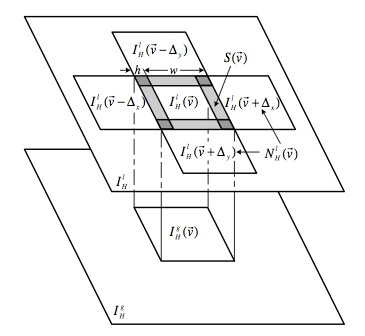
\includegraphics[width=2.5in]{markov.jpg}

\caption{Markov Network as in \cite{Liu}}
\label{fig_sim}
\end{figure}
\begin{equation}
E_G^{ext}(\overrightarrow{v}) = \frac{1}{\lambda'}\sum_{i=1}^k\delta[I_H^l(\overrightarrow{v})-I_H^{l(i)}(\overrightarrow{v})]d^2[I_H^g(\overrightarrow{v}),I_H^{g(i)}(\overrightarrow{v})]
\end{equation}
The $\lambda'$ in this function is the variance which is a preset scalar. Then for each image in the training set of size $K$, we take the Dirac of the difference between the patch at position $v$ in the training image $i$ and the patch at the same position in the image from step 1. The product of this multiplication with the norm sum of squared differences of the Laplacian for the two same patches (one from training image $i$ and one from the output of step 1), is one sum in the entire summation. We can get $E_G^ {ext}$ by summing over these values for each of the training images. In the next step, we want to calculate the internal component. In order to this, we take each patch, one at a time, and  use this equation:
\begin{equation}
E_G^{int}(\overrightarrow{v}) = \frac{1}{\lambda''}\sum_{\mathbf{u}\in S(\overrightarrow{v)}}[I_H^l(\mathbf{u}) - N_H^l(\mathbf{u})]^2
\end{equation}
As described in the paper, each patch at position $v$ has a set of neighbors $S$. The internal function for that patch is the sum of the squared differences between itself and each of its neighbors. Note that in some cases a patch may have only $2$ or $3$ neighbors only if it is on the edge of the image. Also, the patches themselves overlap their neighbors by a few pixels. This is done so that the resulting final image does not look like a collage with visible edges between patches. Thus, in this model, not only is influence propagated via the Markov network but also because the patches actually have pixels common to them, the assignment to the peripheral pixels for one patch is exactly the same as for the other.\\
With this step we get the two components of the Gibbs function which need to be added together. Once we have this for each patch, summing over this values of this function for each patch will provide us the total energy for the Markov network. Finally, minimizing this energy using a MAP algorithm such as Max product will output the final result. Note, in addition to what we have understood and explained here, \cite{Liu} in their implementation have used some other subtle techniques such as simulated annealing which have no understanding of. Additionally, while they loop through the patches they have talked about flipping every patch in the candidate output image, but to what end, we could not exactly understand. 


\section{Implementation \& Issues}
In this section we aim to describe the approach that we have taken in implementing the methods and concepts described above, along with the challenges that we faced in doing so.\\
\subsection{Global Constraint}
We implemented this part successfully, as can be seen from the code submitted. The code is in MATLAB as it was easy to perform the many matrix operations that were required. The variables have been named as they appear in \cite{Liu} so as to avoid confusion.
The image $I_g^*$ obtained at the end of this stage is dependent of the value of $\lambda$ chosen. We have observed that a value between $0.2$ and $0.3$ gives fair results.
\subsubsection{Issues Encountered}
\begin{itemize}
\item The biggest challenge in this paper was understanding the mathematical notations used.There were some parameters that were not very well-defined and hence caused ambiguity during the implementation. For instance, the concept of representing an image as a $1$-D long vector was difficult to grasp and even harder to implement.
\item PCA as a concept was new to us and we struggled a bit due to the different functions that are available in MATLAB to retrieve the eigenvectors and eigenvalues of a matrix, each having different inputs and outputs (eg: $\mathit{princomp}$ and $\mathit{svd}$).
\item We encountered a problem with MATLAB wherein performing this first step is too slow. We also found that MATLAB tends to run out of memory when more than 20 images are used.
\end{itemize}
\subsection{Local Constraint}
We started implementation of the local constraint part of the face hallucination project but were unable to complete it. This was due to several reasons.
\begin{itemize}
\item We both lacked the experience in working with vision techniques and Markov network related projects. Till date, we had only worked with one Markov network and inference based project which was for a significantly simpler Markov network.
\item We felt that the Markov Network described in the local constrain part of the paper was overly complicated and involved many terms, and techniques that we were totally unfamiliar with.

\end{itemize}
However, we did write some code for this part which does not really output anything tangible and is a work in progress. The output that our code currently outputs is only a result of the first step. With that said, the contents of our incomplete attempt to implement the local constraint are described as follows. We initialize a $16$x$16$ matrix of many $8$x$6$ matrices. Here each $8$x$6$ matrix is a patch and hence a $128$x$96$ image has $16$x$16$, $8$x$6$ patches. While we iterate over the training images, for each patch we calculate the external part of the Gibbs function as described earlier in the paper, which comprises of the Dirac function and the difference between the Laplacian of two patches. This is stored in the matrix described above at corresponding indexes. We keep adding to it as we iterate over the training images. We could not get around to implementing the internal component of the Gibbs function as we were short on time and decided to focus on writing the paper. 




% An example of a floating figure using the graphicx package.
% Note that \label must occur AFTER (or within) \caption.
% For figures, \caption should occur after the \includegraphics.
% Note that IEEEtran v1.7 and later has special internal code that
% is designed to preserve the operation of \label within \caption
% even when the captionsoff option is in effect. However, because
% of issues like this, it may be the safest practice to put all your
% \label just after \caption rather than within \caption{}.
%
% Reminder: the "draftcls" or "draftclsnofoot", not "draft", class
% option should be used if it is desired that the figures are to be
% displayed while in draft mode.
%


% Note that IEEE typically puts floats only at the top, even when this
% results in a large percentage of a column being occupied by floats.


% An example of a double column floating figure using two subfigures.
% (The subfig.sty package must be loaded for this to work.)
% The subfigure \label commands are set within each subfloat command, the
% \label for the overall figure must come after \caption.
% \hfil must be used as a separator to get equal spacing.
% The subfigure.sty package works much the same way, except \subfigure is
% used instead of \subfloat.
%
%\begin{figure*}[!t]
%\centerline{\subfloat[Case I]\includegraphics[width=2.5in]{subfigcase1}%
%\label{fig_first_case}}
%\hfil
%\subfloat[Case II]{\includegraphics[width=2.5in]{subfigcase2}%
%\label{fig_second_case}}}
%\caption{Simulation results}
%\label{fig_sim}
%\end{figure*}
%
% Note that often IEEE papers with subfigures do not employ subfigure
% captions (using the optional argument to \subfloat), but instead will
% reference/describe all of them (a), (b), etc., within the main caption.


% An example of a floating table. Note that, for IEEE style tables, the 
% \caption command should come BEFORE the table. Table text will default to
% \footnotesize as IEEE normally uses this smaller font for tables.
% The \label must come after \caption as always.
%
%\begin{table}[!t]
%% increase table row spacing, adjust to taste
%\renewcommand{\arraystretch}{1.3}
% if using array.sty, it might be a good idea to tweak the value of
% \extrarowheight as needed to properly center the text within the cells
%\caption{An Example of a Table}
%\label{table_example}
%\centering
%% Some packages, such as MDW tools, offer better commands for making tables
%% than the plain LaTeX2e tabular which is used here.
%\begin{tabular}{|c||c|}
%\hline
%One & Two\\
%\hline
%Three & Four\\
%\hline
%\end{tabular}
%\end{table}


% Note that IEEE does not put floats in the very first column - or typically
% anywhere on the first page for that matter. Also, in-text middle ("here")
% positioning is not used. Most IEEE journals/conferences use top floats
% exclusively. Note that, LaTeX2e, unlike IEEE journals/conferences, places
% footnotes above bottom floats. This can be corrected via the \fnbelowfloat
% command of the stfloats package.






% use section* for acknowledgement
\section{Conclusion}
We struggled a lot to understand this paper from the start as it was quite advanced relative to our knowledge and understanding of this field. However, we learned a lot at every step of it. We definitely felt like we bit more than we could chew given the scope and time-frame. Ironically, although this was meant to be an exercise in probabilistic models for us, we could not get around to the part where we implemented the actual Markov networks. Yet, we learned a lot of things from imaging, vision and linear algebra, that often go hand in hand with probabilistic models. Overall, while we did not get satisfactory tangible results, it was a really great satisfying and enriching learning experience for the both of us.




% trigger a \newpage just before the given reference
% number - used to balance the columns on the last page
% adjust value as needed - may need to be readjusted if
% the document is modified later
%\IEEEtriggeratref{8}
% The "triggered" command can be changed if desired:
%\IEEEtriggercmd{\enlargethispage{-5in}}

% references section

% can use a bibliography generated by BibTeX as a .bbl file
% BibTeX documentation can be easily obtained at:
% http://www.ctan.org/tex-archive/biblio/bibtex/contrib/doc/
% The IEEEtran BibTeX style support page is at:
% http://www.michaelshell.org/tex/ieeetran/bibtex/
%\bibliographystyle{IEEEtran}
% argument is your BibTeX string definitions and bibliography database(s)
%\bibliography{IEEEabrv,../bib/paper}
%
% <OR> manually copy in the resultant .bbl file
% set second argument of \begin to the number of references
% (used to reserve space for the reference number labels box)
\begin{thebibliography}{1}

\bibitem{Liu}
Ce Liu, Heung-Yeung Shum,Chang-Shui Zhang \emph{A two-step approach to hallucinating faces: global parametric model and local nonparametric model},Computer Vision and Pattern Recognition, 2001. CVPR 2001. \emph{Proceedings of the 2001 IEEE Computer Society Conference on , vol.1, no., pp.I-192,I-198 vol.1}, 2001
\bibitem{Baker}
Simon Baker,Takeo Kanade \emph{Hallucinating Faces}, 2000
\bibitem{Yang}
Jianchao Yang, Hao Tang, Yi Ma, Thomas Huang \emph{Face Hallucination via Sparse Coding},2008
\bibitem{Freeman}
Bill Freeman and Ce Liu, \emph{Markov Random Fields for Super-resolution and Texture Synthesis}, 2010

\end{thebibliography}




% that's all folks
\end{document}


